% Developer documentation
\part{Fejlesztői dokumentáció}

\subsection{Felhasznált technológiák}
A szakdolgozatomat eclipse fejlesztőkörnyezetben írtam, amelyet végül mavennel fordítottam ki és csomagoltam be. A szakdolgozat felhasznál egy külső könyvtárat \cite{hand_eval}, amely a nyertes kiértékelési feladatát látja el. A programcsomagot meg kellett támogatni egy adatbázissal is - MySQL - , amely az adatok perzisztens tárolásáért felel. A programcsomag szerver-kliens architektúrában került implementálásra, amely kliens oldalon tovább bomlik MVC (Model-View-Controller) tervezési stílusra. A szerver és a kliens közötti kommunikáció RMI Java API felhasználásával történik. A maven, mint build system nagyban hozzájárult a programcsomag modernkori elvárások megfeleléséhez, mint például a kód dokumentálásához és a programcsomag disztribúciójához. Igyekeztem áttolni a fejlesztési nehézségeket a felhasznált technológiák vállára. Így például, ha valamilyen oknál fogva friss adatbázisra volt szükségem, akkor azt a
 \begin{verbatim}
mvn clean install -Pbootstrap
\end{verbatim}
parancs kiadásával érhettem el.

\subsection{Adatbázis séma}
\begin{figure}[h!]
  \caption{Adatbázis séma}
  \centering
    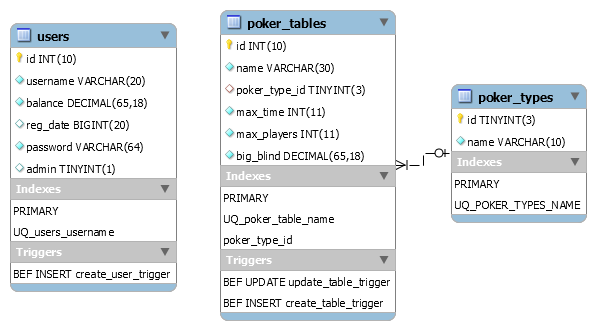
\includegraphics[width=\textwidth]{user-documentation/images/db_scheme.png}
\end{figure}
Az adatbázis (ld. X. ábra) 3 táblából épül fel
\begin{itemize}[leftmargin=2.7cm]
\item users
\item poker\_tables
\item poker\_types
\end{itemize}
 Minden tábla rendelkezik elsődleges kulcssal, amelynek típusa UNSIGNED INTEGER, kivétel a poker\_types táblát, ugyanis ennek a táblának az elsődleges kulcsa UNSIGNED TINYINT típusú, amelyet a MySQL Server 4 byteon tárol. Az adatábrázolás mértékének a szűkítése ebben az esetben indokolt, ugyanis a 255 különböző értékű UNSIGNED TINYINT típus kielégíti a játéktípusok által támasztott követelményeket. A játékstílusok neveit is el kell tárolni, amelynek a maximális hossza 10 karakterben lett meghatározva, amely triggerrel van védve. A users tábla tartalmazza a regisztrált felhasználókat. A regisztrált felhasználók felhasználónévvel és jelszó párossal tudnak regisztrálni, és ennek megfelelően ezek az adatok tárolásra is kerülnek. A felhasználónév maximális hossza 20 karakter, ameyelet triggerrel ellenőrzök. A jelszót bcrypt függvénnyel nyírom. Só eltárolása nem szükséges a bcrypt implementációjából adódóan. A felhasználóról el kell még tárolni a regisztráció dátumat, amely a szerver ideje alapján számolódik és UNIX timestampként kerül letárolásra, továbbá a jogosultsági (admin) szintet, amely ugyancsak 4 byteon (TINYINT) kerül ábrázolásra. A 0/1 értékek megfeleltethetőek a TRUE/FALSE logikai típusú konstans értékeknek, így tehát, ha az érték 0, vagyis FALSE, akkor az adott felhasználó nem rendelkezik admin jogkörrel, különben igen. Ugyancsak tárolandó érték a felhasználó játékbeli egyenlege, amely BIGDECIMAL típúsként van ábrázolva.
A játéktáblákat a poker\_tables adatbázis tábla tárolja. Szükségünk van eltárolni a játéktábla nevét, melynek felső korlátja 30 karakter és egyedinek kell lennie. Ezeket a megszorításokat szintén triggerekkel ellenőrzöm. A játék asztal játékstílusát is eltárolom, amely egyben idegenkulcs is a poker\_types táblára nézve. Továbbá minden asztal tulajdonsága, hogy maximum hányan játszhatnak rajta, és hány másodpercig gondolkodhatnak a játékosok. Ezen két érték típusaként ugyancsak UNSIGNED TINYINT van meghatározva, ugyanis az egyes asztaloknál a játékosok száma legfeljebb 5 lehet, míg az egyes játékosok gondolkodási ideje maximum 40, de legalább 5 másodperc.

\subsection{Modulok}
A programcsomag 6 fő modult tartalmaz
\begin{description}
  \item[poker-server] \hfill \\
  A póker játék szervere, amely magát a játékot szolgáltatja.
  \item[poker-client] \hfill \\
  A póker játék kliense, amely segítségével a szerverhez lehet csatlakozni.
  \item[poker-shared] \hfill \\
   A póker játék azon modulja, amelytől a szerver és a kliens egyaránt függ.
   \item[poker-persist] \hfill \\
   Az adatok letárolásáért felelős modul.
   \item[poker-model] \hfill \\
   A póker játék modellezéséért felelős csomag.
   \item[javapokertexasholdem] \hfill \\
   Külső könyvtár, amely a nyertes játékos kiértékelési feladatot végzi.
\end{description}
\begin{figure}[h!]
	\caption{Kliens modulra bontása}
	\label{fig:client_modul}
	\centering
	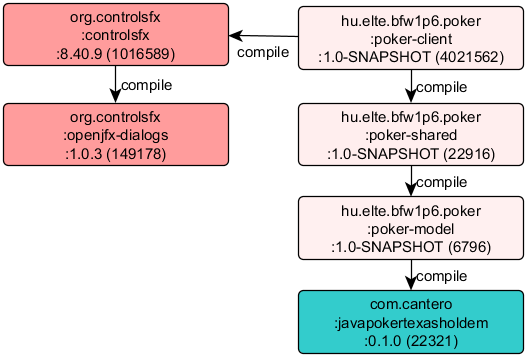
\includegraphics{user-documentation/images/poker-client-deps.png}
\end{figure}
\begin{figure}[h!]
	\caption{Szerver modulra bontása}
	\label{fig:server_modul}
	\centering
	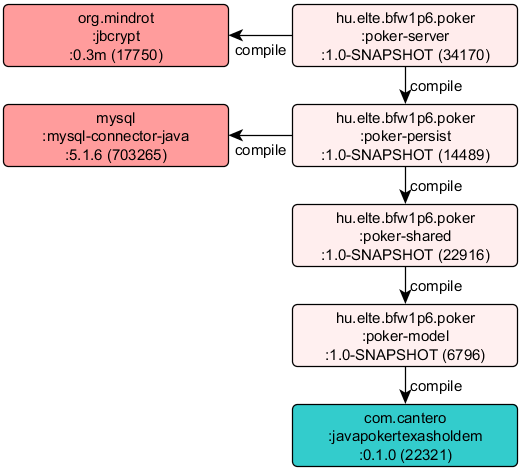
\includegraphics{user-documentation/images/poker-server-deps.png}
\end{figure}
A modulok közötti függőséget a \ref{fig:client_modul}. és a \ref{fig:server_modul}. ábra szemlélteti. \\
A programcsomag két főmodulra bontható
\begin{itemize}[leftmargin=2.7cm]
\item poker-server
\item poker-client
\end{itemize}

\subsubsection{Model} \label{sec:poker-model}
A poker-model modul felelős a játék modellezésért. A X. ábrán látható a modul felépítése. Az entitásokat össze kellett fogni az EntityWithId interfész segítségével, ezáltal a DAO (későbbi képre hivatkozás...?) objektumot generikusan lehetett megfogalmazni, amely segített a kód duplikációk elkerülésében. A PokerTable és a User osztályok példányai feleltethetőek meg a poker\_tables és a users adattáblák egyes rekordjainak. A PokerType enumeráció a játékstílusokat határozza meg. Ha egy új játékstílust szeretnénk hozzáadni a játékhoz, akkor a kódban egy új PokerType enum objektumot kell felvennünk, és a poker\_schema.sql állományban pedig fel kell venni egy új insert utasítást a poker\_types táblára nézve az új játékstílus nevére vonatkozólag. Természetesen ez a pár sor újonnan hozzáadott kód nem azt jelenti, hogy már használhatjuk is az új játékstílust. A programcsomagot több ponton is ki kell bővíteni
\begin{itemize}[leftmargin=2cm]
	\item Szerver oldal
		\begin{enumerate}
			\item AbstractPokerTableServer osztályt ki kell terjeszteni egy új osztállyal
		\end{enumerate}
	\item Kliens oldal
		\begin{enumerate}
			\item Új leszármazott osztályokat kell létrehozni a kliens oldali MVC absztrakciós osztályaiból (ld. később) vagy hivatkozva...
			\item Új fxml állományt kell létrehozni
		\end{enumerate}
\end{itemize}

\subsubsection{Shared}
A poker-shared modul olyan közös osztályokat tartalmaz, amelyeket a kliens és a szerver egyaránt használ. Itt helyezkednek el az egyéni kivételek, a kommunikációs rendszer definíciója és a kliens, mint megfigyelő interfésze.

\pokerparagraph{Kivételek}
A játékcsomagnak szüksége van egyéni kivételekre. Az olyan speciális eseteket, mint például adabázisba írás, illetve abból olvasás közbeni fellépő kivételt saját kivételobjektumokkal célszerű lekezelni. Ehhez hasonló egyéni kivételek fellépthetnek bejelentkezéskor, asztalhoz való csatlakozáskor, hibás jelszó megadás esetén, stb (ld. melléklet, javadoc...).

\pokerparagraph{Kommunikációs rendszer}
A szerver és a kliens  üzeneteket küldhetnek egymásnak. \\
Ide jöhet a kép... Az ún. messaging systemet igyekeztem minél absztraktabb módon megfogalmazni, ezzel is elősegítve a későbbi bővíthetőségi nehézségeket. Azonban sajnos helyenként fellelhető kód duplikáció az enumerációkra való építkezés miatt. \\
Minden utasításnak kötelezően implementálnia kell a PokerCommand interfészt, ezzel is elősegítve az általános megfogalmazást a rendszerben. Két fajta utasítás létezik a játékcsomagban:
\begin{itemize}[leftmargin=2cm]
	\item Szerver utasítás
	\item Kliens utasítás
\end{itemize}
Továbbá a játékstílusnak megfelelően tovább szigorodik... (kéne egy jó szó) a küldendő üzenet fajtája. A programcsomag kettő játékstílust fogalmaz meg (ld. \ref{subsubsec:game_styles}). A játékstílusok különböző utasítás fajtákat igényelnek. Értelemszerűen, ha egy Holdem játékstílusban résztvevő kliens üzenetet szeretne küldeni a játék asztal szervernek , akkor egy HoldemPlayerCommand típusú objektumot kell elküldenie a szerver csonkon keresztül. \\
Az üzeneteknek vannak fajtái, amelyeket a mellékletben meg lehet tekinteni.

\pokerparagraph{Observer pattern \cite{observer_pattern}}
Az oberserver tervezési minta segítségével megvalósítható RMI API-n keresztül az ún. event driven server. Így nem csak a kliens tud üzenet küldeni a szervernek, hanem a szerver is tudja értesíteni a klienseket. Például, ha egy játékos CHECK típusú utasítást küldött a szervernek (játékstílustól függetlenül), akkor azt az üzentet a szerver minden kliensnek szétszórja (broadcast, üzenetszórás... valahogy jól kéne megfogalmazni).

\pokerparagraph{Session}
% ez a szöveg lehet, hogy server modulba kéne....
A szerver a klienseket session objektumokkal azonosítja. Minden kliens kap egy sessiont a bejelentkezéskor. A session addig él, amíg a felhasználó ki nem jelentkezik, akkor ugyanis a munkamenet érvénytelenítésre kerül. Illetőleg a munkamenetet akkor is érvényteleníteni kell, ha a kliens nem jelentkezett ki, de a kapcsolat valamilyen oknál fogva megszakadt. \\
Amikor egy kliens be szeretne jelentkezni a játékba, akkor a szerver az összes megszakadt kapcsolatú klienst felderíti, és a munkamenetüket érvénytelennek tekinti. A felderítés ún. pingeléssel történik. A szerver minden csatlakozott klienst megpróbál elérni, és amelyik kliensnél megszakadt a kapcsolat, azt eltávolítja a szerverről. Ezután a SessionService ellenőrzi, hogy az adott felhasználónévvel van-e aktív munkamenet, ha van, akkor kivételt dob az eljárás, különben az autentikáció sikeres, és a kliens oldali model eltárolja a loginkor kapott sessiont.
\subsubsection{Persist}
A poker-persist modul látja el az adatbázissal kapcsolatos teendőket. Ez a modul írja és olvassa az adatbázist a bejövő kérések és paraméterek alapján.
\pokerparagraph{Generikus DAO}
A generikusság elengedhetett a kódismétlés elkerülése végett. Általánosan kell megfogalmazni az entitások viselkedését \ref{sec:poker-model} (vagy fordítva...), és ezáltal a persist modul letisztult arculatot kap. A GenericDAO osztály tartalmaz minden olyan elemet, amelykre a specializálódott DAO-knak szükségük lehet.
\pokerparagraph{Adatbázis menedzser}
Az AbstractDAO-nak szükséges van tényleges adatbázis kapcsolatra, amelyet a DBManager osztály szolgáltat.
\pokerparagraph{Kivételek átfordítása}
Az AbstractDAO rendelkezik egy SQLExceptionTranslator objektummal is, amely az adatbázisból érkező hibát fordítja át PokerDataBaseException típusú kivételre. A PokerDataBaseException kivétel osztály a felhasználó számára is értelmes hibaszöveget hordoz magában.

\subsubsection{Kliens}
A kliens modult és annak minden függőségét egy jar fileba csomagolva kell szétterjeszteni a felhasználók között, akik majd ténylegesen használni fogják a programot. A \ref{fig:client_modul}. ábra alapján a jar file tartalmazni fog minden olyan osztályt és interfészt, amelyre ténylegesen szüksége lesz a kliens programnak. Az összecsomagoláshoz igénybe vehetjük a mavent és annak az assembly pluginját. A poker-client könyvtárban a
 \begin{verbatim}
mvn clean compile assembly:single
\end{verbatim}
paranccsot kiadva a poker-parent/release könyvtár alá csomagolódik be a futtatható jar állomány. \\
\pokerparagraph{Model-View-Controller \cite{MVC}}
Az igen közkedvelt tervezési minta alapján valósítottam meg a kliens oldali programot.
\subparagraph
Model \\
lol


\subsubsection{Szerver}
\subsubsection{javapokertexasholdem}

\pokerparagraph{Szerver}
\begin{figure}[h!]
  \caption{A szerver publikus interfésze}
  \label{fig:server_public}
  \centering
    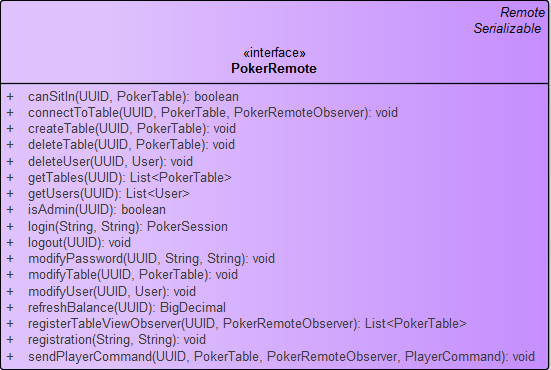
\includegraphics[width=\textwidth]{user-documentation/images/server_remote.png}
\end{figure}
A szerver feladata a játék biztosítása a kliensek számára. A \ref{fig:server_public}. ábrán látható a szerver jóldefiniált publikus interfésze. A kliensek ezt az interfészt tudják elkérni a registryből \cite{RMI}

A szerver a jelszavak titkosítására bcrypt eljárást alkalmaz, amelynek a biztonságát sózással növeli. Továbbá a szerver felhasznál még egy külső csomagot - mysql-connector-java -, amely az adatbázis kapcsolatért felel.
A poker-shared modul felel a szerver és a kliens jól definiált kommunikácójáért. A shared modul többek között tartalmazza a közös interfészeket, kivételeket és a póker utasítások megvalósítását. A kliens közvetlenül függ ettől a modultól, azonban a szerver és a shared modul közé beékelődött a poker-persist modul, amely az adatok adatbázisba való írásáért és abból olvasásáért felel.

\subsection{Funkciók}
Ahogy a témabejelentőben is szerepel...... RMI kép wikiről, majd azt megmagyarázni a shared modullal, kliens hívja, jól definiált interfész etc....
\begin{figure}[h!]
	\caption{RMI koncepció}
	\centering
	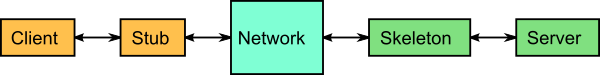
\includegraphics[width=14cm, height=2cm]{user-documentation/images/rmi.png}
\end{figure}
A szerver vázáért a PokerRemote interface felel, amely a játékon végrehajtható műveletek összefogásáért felel. Itt található az összes funkció, amely megvalósításra került, mint például játék asztal létrehozása, új felhasználó létrehozás, admin jog kiosztása stb. A kliens ezt a vázat tudja elkérni az RMI registryből, mint kliens-oldali szervercsonk, amelyeken a műveletek meg tudja hívni. Az összes megvalósított funkciót le kell írni? Felsorolás szintjén, vagy hogy? Rövid magyarázattal? És amelyik egyértelmű? Pl. felhasználó módosítása... login...

\subsection{Tovább fejlesztési lehetőségek}
\begin{itemize}
\item Az adatbázis viszonylag alacsony absztrakciós szinten került implementására, azonban mivel néhány tábláról beszélhetünk csak, ezért igyekeztem elkerülni a keretrendszerek általi overheadet. Ugyanakkor ezen a ponton sokat fejlődhet a programcsomag, ha a későbbiek során esetlegesen bonyolultabban kellene modellezni a játékot adatbázis szempontjából. Például dialektusok - akár Liquibase (hivatkozás) - használata elfedheti a tényleges adatbázis-kezelő rendszer általánosságait, így eggyel magasabb szintre helyezhető a megvalósítás.
\item A felhasználói élményen sokat javíthat az animációk használata. A megjelenítés sokkal lágyabb, folyékonyabb lehetne Transition/Animation (bibliográfiába hivatkozás...) objektumok használatával.
\item Akár a komplett RMI architektúrát le lehetne váltani, és helyette REST szoftverarchitektúrát alkalmazni, amely modernebb megjelenést (AngularJS, reszponzív design) és modernebb fejlesztői eszközöket, API-kat vonna maga után.
\item A játék nem képes kezelni olyan eseteket, amikor egynél több játékos nyer az adott körben.
\item A játék nincs felkészítve arra a szélsőséges esetre, ha valakinek elfogy a zsetonja, akkor pontosan minek (és hogyan) kell történnie.
\item A kódban viszonylag sok kód duplikáció van jelen, ugyanis az HouseCommandType és a PlayerCommandType enum típusú objektumok szűk keresztmetszetnek tudható be. Ha a PokerCommand interfacet implementáló osztályokat generikusan tudnánk megfogalmazni, akkor jelentősen letisztulna a kód.
\item Az admin jogot el lehetne távolítani a játékból, és helyette MVC tervezési minta alapján a szerver oldalra is implementálni lehetne egy grafikus interfészt, amelyen keresztül a szerver teljeskörű karbantartása és adminisztrációja elvégezhető lenne.
\end{itemize}

\subsection{Tesztelés}
\subsubsection{Funkcionális tesztelés}
\begin{tabular}{| l | c | r |}
\hline
  Funkció & Elvárt eredmény & Eredmény \\ \hline
  Regisztráció & A program jelezte a felhasználónak, hogy a regisztráció sikeresen megtörtént, és visszairányította őt a bejelentkezési formhoz. & A felhasználó a regisztrációt követően be tudjon jelentkezni a póker játékba. \\ \hline
  Bejelentkezés & A formot helyesen kitöltve a program sikeresen autentikálta és beléptette a felhasználót. & Regisztrációt követően be tudjon jelentkezni a felhasználó \\ \hline
  Tábla módosítás & - & - \\ \hline
  Tábla törlés & - & - \\ \hline
\end{tabular}


\clearpage
